\documentclass{aa}

% \usepackage[utf8x]{inputenc}
% \usepackage[T1]{fontenc}
% \usepackage{txfonts, natbib}
% \usepackage{amsmath, amsfonts, amssymb}
\usepackage{graphicx}

\begin{document}

\title{Dynamical evidence of the age--metalicity relation in the Milky Way disk \thanks{This paper is based on data collected at the Observat\'orio Pico dos Dias, operated by Laborat\'orio Nacional de Astrof'{\i}sica, MCT, Brazil.}}

\author{
    H. J. Rocha-Pinto\inst{1}
    \and R. H. O. Rangel \inst{1}
    \and G. F. Porto de Mello \inst{1}
    \and W. J. Maciel \inst{2}
}

\offprints{H. J. Rocha-Pinto}

\institute{OV \and IAG}

\titlerunning{Dynamical evidence of the age--metalicity relation}
\authorrunning{H. J . Rocha-Pinto}

\date{Received date; accepted date}

\abstract
% context
{This is context}{This is aim}{This is methodology}{This is results}{This is conclusion}

\keywords{Galaxy: evolution -- stars: late-type -- solar neighbourhood}

\maketitle

\begin{figure}
    \resizebox{\hsize}{!}{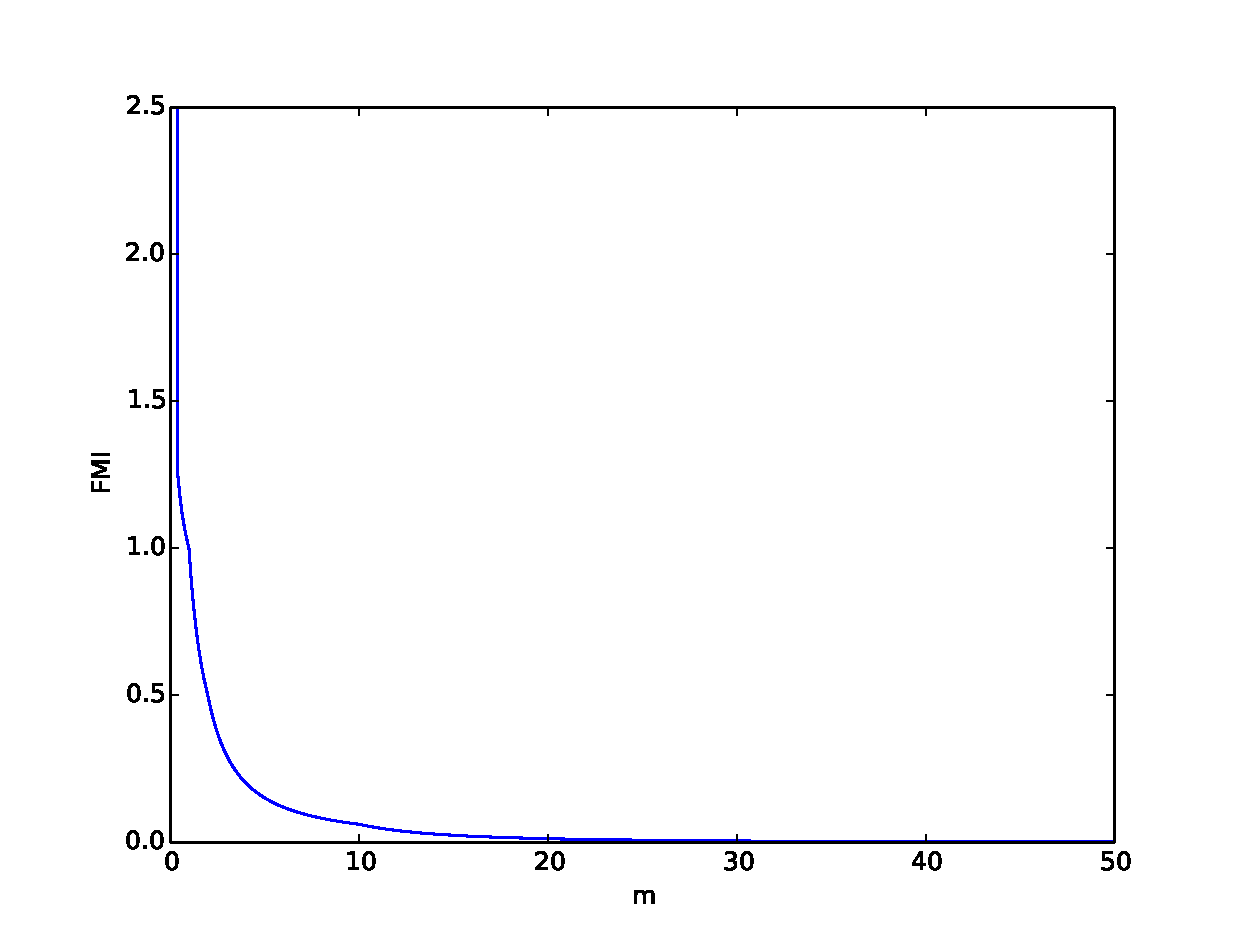
\includegraphics{figs/f4.eps}}'
    \caption[]{Average abundance of Fe, Na, Si, Ca, Ni, and Ba as ...}
    \label{ztrend}
\end{figure}

\end{document}
